\documentclass[../../main.tex]{subfiles}

\lstset{basicstyle=\small,
      showstringspaces=false,
      commentstyle=\color{black},
      keywordstyle=\color{blue}
    }

\graphicspath{{images/Signalerkennung/}{../../images/Signalerkennung/}}


\begin{document}
\subsection{Signalerkennung}
    In der Aufgabenstellung wird gefordert, dass der Schnellzug während der Bewältigung der Strecke ein Signal mit aufgedruckter Nummer erkennt wird. Wie in der Abbildung XX ersichtlich, ist die Nummer auf einer 3x3cm Tafel mit weissem Hintergrund, schwarz aufgedruckt. Die Aufgabe Signalerkennung wird in zwei Teilaufgaben unterteilt:
    \begin{itemize}
        \item Erkennung der Signalisation mit Tafel
        \item Erkennung der aufgedruckten Nummer
    \end{itemize}
    Wie bereits in der Übersicht beschrieben, wird im Gesamtkonzept zwei Kameras verwendet. Eine Kamera wird zur Erkennung der Gleisrichtung verwendet. Die zweite Kamera wird nun für die Signalerkennung eingesetzt. Der Raspberry PI 3+, welcher als Hauptrecheneinheit geplant ist, verfügt nur über einen CSI- Anschluss (Camera Serial Interface). Für die Signalerkennung wird daher auf einen weiteren kleineren Raspberry PI Zero W gesetzt. Dieser verfügt wie der Raspberry PI 3+ einen vollwertigen CSI- Anschluss und kann somit die zweite Kamera bedienen. Dies führt auch dazu, dass der Raspberry PI 3+ zusätzlich entlastet werden kann.\\

    \textbf{Architektur}\\
    Die Signalerkennung in zwei Teilaufgaben zu trennen hat noch einen weiteren vorteil. Die beiden Teilaufgaben werden auf beide Raspberry PIs verteilt. Der Raspberry PI Zero W ist für die Bilderaufnahme Verarbeitung und für die Signalerkennung mit Tafel zuständig. Der Raspberry PI 3+ übernimmt dann die Erkennung der aufgedruckten Nummer auf der Tafel. So kann die Ressourcen des Raspberry PI 3+ gezielter eingesetzt werden.

    \begin{figure}[H] %Architektur
        \centering
        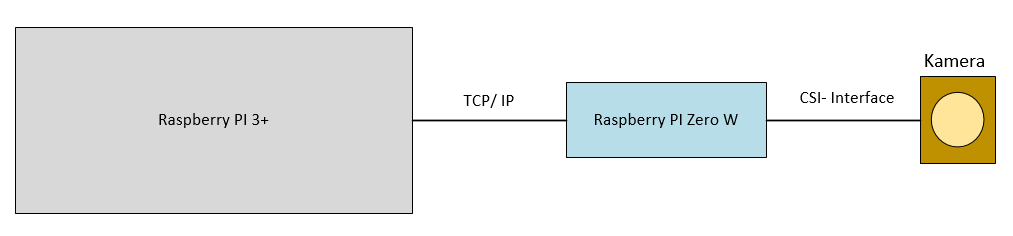
\includegraphics[width=0.9\textwidth]{Architektur.png}
        \caption{Architektur Hardware Signalerkennung}
        \label{fig:architektur_hardware_signalerkennung}
    \end{figure}

    Für die Nummererkennung auf der Tafel wird ein auf Keras und Tensorflow basierender Machine- Learning Algorithmus verwendet. Damit die Trainingsdaten des Models eingelesen werden können und somit Tenserflow ausführbar wird, braucht es eine gewisse grösse des Arbeitsspeichers. Der Arbeitsspeicher des Raspberry PI Zero W (512Mb) reicht dafür nicht aus. Der Raspberry PI 3+ verfügt über mehr speicher (1Gb) und kann somit den Algorithmus bearbeiten. Für die Kameraufnahmen und die Bearbeitung der Bilder und schlussendlich die Konturenerkennung der Signalisation ist der Raspberry PI Zero W gut geeignet. 




\end{document}